% !Mode:: "TeX:UTF-8" 
\section{前期的理论研究与实验论证工作的结果}

本课题相关的理论研究始于2015年11月,在经过深度调研语义依存分析及与其相关的其它自然语言处理技术的基础上,开始研究如何利用基于转移的分析方法实现对语义依存图的分析。我们首先使用最直观的方法实现了一个基准模型,即将该任务分为两步,第一步用传统依存树分析器生成依存树结构,然后通过后处理将该依存树转换成语义依存图。然后又分别提出了两个能够直接生成依存图结构的转移系统,并借鉴了\citeayu{chen2014acl}的思路,用MLP作为系统的分类器预测转移动作,在SemEval-2016 Task 9中文语义依存图数据集上取得了当时最好实验结果。这部分工作已被CCL 2016收录,并获得当年最佳论文奖。

此后,为了进一步提高基于转移的依存图分析器的性能,我们受\citeayu{dyer-EtAl:2015:ACL-IJCNLP}工作的启发,利用栈-长短时记忆网络(Stack LSTM)从转移系统中更全面地学习用于预测的信息,同时提出了Bi-LSTM Subtraction和Incremental Tree-LSTM两种结构分别学习缓存(buffer)和系统中子图更好的表示,然后综合利用这些信息进行转移动作的预测,在中文语义依存图数据集上刷新了最好实验结果,同时在SemEval-2015 Task 18的英文语义依存图数据集上也取得了与最好系统相近的结果。该工作已经被AAAI 2018录用。本文将主要介绍以下两篇工作:

\begin{enumerate}
	\item Transition-Based Chinese Semantic Dependency Graph Parsing. (CCL2016, 已发表)
	\item A Neural Transition-Based Approach for Semantic Dependency Graph Parsing. (AAAI 2018, 已发表)
\end{enumerate}


\subsection{基于转移的语义依存图分析技术研究}
\subsubsection{实验动机}

由于结构上的相似之处,现阶段语义依存图分析的主要方法都来自于对依存句法分析领域内的基于转移和基于图的两类方法的扩展。在基于图的分析方法中,首先要算出各个可能的子结构的分数,然后计算总分最大的组合(这一步称为解码过程)。对于树结构和图结构来说,第一步基本没有区别,但在第二步解码过程中,目标结构的不同使得二者变成了完全不同的解码问题。现有方法或者先生成树,再通过后处理将其转化成图\citeyqy{mcdonald2006online},或者只能采用新的解码算法\citeyqy{martins2014priberam,peng-thomson-smith:2017:Long}。

相对来说,在基于转移的分析方法中,通过修改现有转移系统,增删或修改转移动作\citeyqy{sagae2008shift, Titov:2009:OGP:1661445.1661696, Zhang:2016:TPD:3030588.3030589}就能实现依存图结构的分析,实际上只需要增加预测转移动作的分类器类别。因此,我们选择基于转移的分析方法作为突破口,提出新的转移系统实现直接产生语义依存图。此外,前人的此类工作中普遍使用了最大熵模型\citeyqy{ratnaparkhi1997simple}、结构化感知器\citeyqy{collins:2002:EMNLP02}等传统统计学机器学习方法预测转移动作。这类方法需要人工进行特征模板的设计,不仅费时费力、需要本领域专家知识,而且往往难免遗漏一些信息,同时特征字符串的组合也会浪费大量时间。所以我们将具有强大信息总结、抽象能力的神经网络作为分析系统中的分类器用于转移动作的预测,解决了上述诸多问题,同时有效提高了语义依存图分析系统的性能。

\subsubsection{方法设计}

基于转移的分析方法通过执行一系列从初始转移状态到终止转移状态的移进、规约等转移动作,实现目标结构的生成。这类方法由两个重要部分组成,一是转移系统,它定义了存放句中词的结构、转移动作集合以及转移动作执行的规则;二是分类器,它以当前转移状态为依据,预测出下一步要执行的转移动作。基于转移的分析方法的核心就是训练一个好的分类器,使得当我们按照它预测的动作产生语义依存图时,与正确的语义依存图尽可能相似。接下来分别介绍我们已经实现的用于分析语义依存图的转移系统和分类器。

\subsubsection*{转移系统}

由于语义依存图具有非投射性(弧之间存在交叉),在设计转移系统时,我们参考了\citeayu{choi-palmer:2011:ACL-HLT2011, choi-mccallum:2013:ACL2013}提出的用于分析非投射依存树的转移系统,并对其做了改进,使其能够直接分析语义依存图。其主要思想是在找到一个词的父节点之后,不再马上将其从转移系统中删除(由于在树结构中,一个词只有一个父节点,因此在分析依存树时,一旦找到了一个词的父节点,就会立即将其从转移系统中删除),而是仍然将其保存在系统中,这样未来这个词就能找到其它的父节点。

\begin{table}[htbp]
	\centering
	\begin{tabular}{l|ll}
		\hline
		\bf 转移动作 \ \ \ \ & \bf 当前转移状态 & $\Rightarrow$ \bf 下一转移状态 \\
		\hline\hline
		Left$_l$-Reduce &\ \ $([\sigma|i],\,\delta,\,[j|\beta],\,A)$ & $\Rightarrow (\sigma,\,\delta,\,[j|\beta],\,A\,\cup\,\{(i\xleftarrow{l}j)\})$ \\
		Right$_l$-Shift &\ \ $([\sigma|i],\,\delta,\,[j|\beta],\,A)$ & $\Rightarrow ([\sigma|i|\delta|j],\,[\ ],\,\beta,\,A\,\cup\,\{(i\xrightarrow{l}j)\})$ \\
		No-Shift &\ \ $([\sigma|i],\,\delta,\,[j|\beta],\,A)$ & $\Rightarrow 
		([\sigma|i|\delta|j],\,[\ ],\,\beta,\,A)$ \\
		No-Reduce &\ \ $([\sigma|i],\,\delta,\,[j|\beta],\,A)$ & $\Rightarrow (\sigma,\,\delta,\,[j|\beta],\,A)$\\
		\hline
		Left$_l$-Pass &\ \ $([\sigma|i],\,\delta,\,[j|\beta],\,A)$ & $\Rightarrow (\sigma,\,[i|\delta],\,[j|\beta],\,A\,\cup\,\{(i\xleftarrow{l}j)\})$\\
		Right$_l$-Pass &\ \ $([\sigma|i],\,\delta,\,[j|\beta],\,A)$ & $\Rightarrow (\sigma,\,[i|\delta],\,[j|\beta],\,A\,\cup\,\{(i\xrightarrow{l}j)\})$\\
		No-Pass &\ \ $([\sigma|i],\,\delta,\,[j|\beta],\,A)$ & $\Rightarrow (\sigma,\,[i|\delta]	,\,[j|\beta],\,A)$\\
		\hline
	\end{tabular}
	\caption{List-based Arc-eager转移系统中的转移动作集合}
	\label{tbl:actions}
\end{table}

\begin{table}[t]
	\small
	\centering
	\begin{tabular}{l|l|l}
		\hline
		\multirow{2}{*}{\bf 动作} & \multicolumn{2}{c}{\bf List-Based Arc-Eager算法中转移动作的执行条件} \\
		\cline{2-3}
		& \bf 依存树分析 & \bf 依存图分析 \\
		\hline
		Le-$*$ & $[i\neq0] \wedge \neg[(i\rightarrow ^*j)\in A] \wedge \neg[\exists k.(i\leftarrow k)\in A] $ & $[i\neq0] \wedge \neg[(i\rightarrow ^*j)\in A] $ \\
		Ri-$*$ & $\neg[(j\rightarrow ^*i)\in A] \wedge \neg[\exists k.(k\rightarrow j)\in A] $ & $\neg[(j\rightarrow ^*i)\in A]$ \\
		$*$-Re & $[\exists h.(h\rightarrow i)\in A] \ \wedge \neg[\exists k\in\beta.(i\rightarrow k)]$ & $[\exists h.(h\rightarrow i)\in A] \ \wedge \neg[\exists k\in\beta.(i\rightarrow k)\vee(i\leftarrow k)]$ \\
		$*$-Sh & \multicolumn{2}{c}{ $\neg[\exists k\in \sigma.(k\neq i) \ \wedge ((k\rightarrow j)\vee(k\leftarrow j))]$ } \\
		\hline
	\end{tabular}
	\caption{依存树分析算法与依存图分析算法转移动作执行条件对比。Le-$*$和Ri-$*$分别表示以Left和Right开头的动作,$*$-Re和$*$-Sh分别表示以Reduce和Shift结尾的动作。}
	\label{tbl:preconditions}
\end{table}

接下来给出该转移系统的正式定义:我们用一个四元组$(\sigma,\delta,\beta,A)$来表示任意一个转移状态,其中$\sigma$是用于保存正在处理中的词的栈;$\delta$是用于保存从$\sigma$中弹出的词的栈,这些词在将来某一时刻将被重新压入$\sigma$中;$\beta$是用于保存等待处理的词的缓存;$A$用于保存已经生成的依存弧。
为了简洁,我们用$i$表示第$i$个词$w_i$,其中$0$表示根节点$w_0$,根据定义,每个依存图的根节点只有一个子节点。初始转移状态是$([0],[\ ],[1,\dots,n],\emptyset)$,终结转移状态是$(\sigma,\delta,[\ ],A)$。
另外,我们用$(i\rightarrow j)$表示一条从$w_i$指向$w_j$的依存弧,其依存关系为$l$。$(i\rightarrow j)$和$(i\rightarrow^*j)$分别表示$w_i$是$w_j$的父节点和祖先节点。
在分析过程中,依存弧只会在栈$\sigma$的顶部元素$w_i$和缓存$\beta$的第一个元素$w_j$之间生成。在训练过程中,转移动作通过标准语义依存图生成,在解码过程中,转移动作通过神经网络分类器预测产生。

\begin{figure}[tb]
	\centering
	\begin{dependency}[theme = simple,label style={font=\bfseries,thick}]
		\begin{deptext}[column sep=0.5em]
			他$_1$ \& 太$_2$ \& 小气$_3$ \& ,$_4$ \& 不$_5$ \& 肯$_6$ \& 请$_7$ \& 我们$_8$ \& 吃饭$_9$ \\
		\end{deptext}
		\deproot{3}{ROOT$_0$}
		\depedge[edge style={red, dashed}, label style={text=red}]{3}{1}{Exp}
		\depedge{3}{2}{mDegr}
		\depedge{3}{4}{mPunc}
		\depedge{3}{7}{eCau}
		\depedge[edge start x offset=6pt, style={red, dashed}, label style={text=red}]{7}{1}{Agt}
		\depedge{6}{5}{mNeg}
		\depedge{7}{6}{mMod}
		\depedge[edge style={red, dashed}, label style={text=red}]{7}{8}{Datv}
		\depedge{7}{9}{ePurp}
		\depedge[edge style={red, dashed}, label style={text=red}]{9}{8}{Agt}
	\end{dependency}
	\caption{中文语义依存图实例,红色虚线表示多父节点情况。}
	\label{fig:csdg0}
\end{figure}

\begin{table*}[thbp]
	\centering
	\small
	\begin{tabular}{C{2em}L{7em}R{4em}C{4em}L{4em}L{9em}}
		\hline
		\bf 状态 & \bf 转移动作 & $\sigma$ & $\delta$ & $\beta$ & $A$ \\
		\hline
		$0$ & Initialization & $[0]$ & $[\ ]$ & $[1, \dots, 9]$ & $\emptyset $ \\
		$1$ & No-Shift & $[0, 1]$ & $[\ ]$ & $[2, \dots, 9]$ &  \\
		$2$ & No-Shift & $[0, 1, 2]$ & $[\ ]$ & $[3, \dots, 9]$ &  \\
		$3$ & Left-Reduce & $[0, 1]$ & $[\ ]$ & $[3, \dots, 9]$ & $A\ \cup\ \{2\leftarrow \textrm{mDegr}-3\}$ \\
		$4$ & Left-Pass & $[0]$ & $[1]$ & $[3, \dots, 9]$ & $A\ \cup\ \{1\leftarrow \textrm{Exp}-3\}$ \\
		$5$ & Right-Shift & $[0, 1, 3]$ & $[\ ]$ & $[4, \dots, 9]$ & $A\ \cup\ \{0- \textrm{ROOT}\rightarrow 3\}$ \\
		$6$ & Right-Shift & $[0, 1, 3, 4]$ & $[\ ]$ & $[5, \dots, 9]$ & $A\ \cup\ \{3- \textrm{mPunc}\rightarrow 4\}$ \\
		$7$ & No-Reduce & $[0, 1, 3]$ & $[\ ]$ & $[5, \dots, 9]$ &  \\
		$8$ & No-Shift & $[0, 1, 3, 5]$ & $[\ ]$ & $[6, \dots, 9]$ &  \\
		$9$ & Left-Reduce & $[0, 1, 3]$ & $[\ ]$ & $[6, \dots, 9]$ & $A\ \cup\ \{5\leftarrow \textrm{mNeg}-6\}$ \\
		$10$ & No-Shift & $[0, 1, 3, 6]$ & $[\ ]$ & $[7, 8, 9]$ &  \\
		$11$ & Left-Reduce & $[0, 1, 3]$ & $[\ ]$ & $[7, 8, 9]$ & $A\ \cup\ \{6\leftarrow \textrm{mMod}-7\}$ \\
		$12$ & Right-Pass & $[0, 1]$ & $[3]$ & $[7, 8, 9]$ & $A\ \cup\ \{3- \textrm{eCau}\rightarrow 7\}$ \\
		$13$ & Left-Reduce & $[0]$ & $[3]$ & $[7, 8, 9]$ & $A\ \cup\ \{1\leftarrow \textrm{Agt}-7\}$ \\
		$14$ & No-Shift & $[0, 3, 7]$ & $[\ ]$ & $[8, 9]$ &  \\
		$15$ & Right-Shift & $[0, 3, 7, 8]$ & $[\ ]$ & $[9]$ & $A\ \cup\ \{7- \textrm{Datv}\rightarrow 8\}$ \\
		$16$ & Left-Reduce & $[0, 3, 7]$ & $[\ ]$ & $[9]$ & $A\ \cup\ \{8\leftarrow \textrm{Agt}-9\}$ \\
		$17$ & Right-Shift & $[0, 3, 7, 9]$ & $[\ ]$ & $[\ ]$ & $A\ \cup\ \{7- \textrm{ePurp}\rightarrow 9\}$ \\
		\hline
	\end{tabular}
	\caption{用List-based Arc-eager算法获得的图~\ref{fig:csdg0}对应的正确转移动作序列.}
	\label{tbl:trans-seq}
	\vspace{-1em}
\end{table*}

后文将该转移系统称为List-based Arc-eager转移系统,其转移动作集合如表~\ref{tbl:actions}所示,事实上,我们仍然沿用了\citeayu{choi-mccallum:2013:ACL2013}的转移动作,但是对其执行条件进行了修改,具体修改见表~\ref{tbl:preconditions}。接下来,通过一个例子进一步说明该转移系统的工作方式,图~\ref{fig:csdg0}是一个中文语义依存图实例,表~\ref{tbl:trans-seq}给出了使用上述转移系统生成该语义依存图的正确转移动作序列。

在状态4时,由于$w_1$在$\beta$中还有另一个父节点$w_7$,它被从$\sigma$中暂时移入$\delta$,它们之间的弧会在未来(即状态13时)再产生。在状态12时,由于$w_7$在$\sigma$中还有一个子节点$w_1$,因此系统执行了Right-Pass动作而不是Right-Shift动作。该动作将$w_3$移入$\delta$从而允许$w_7$和$w_1$之间产生一条弧(在状态13时)。

\subsubsection*{分类器}

如果说转移系统是基于转移的分析方法的骨架,那么分类器就是它的大脑,负责以当前的转移状态为依据决定下一步要执行的转移动作。传统的基于转移的依存分析方法,无论是以图结构为目标的\citeyqy{Titov:2009:OGP:1661445.1661696,sagae2008shift,Zhang:2016:TPD:3030588.3030589},还是以树结构为目标的\citeyqy{yamada2003statistical,nivre-hall-nilsson:2004:CONLL,nivre2008algorithms}普遍使用的都是最大熵模型、结构化感知器等传统感知器模型。这些模型普遍使用百万级别的高维稀疏人工定义特征(例如用01特征函数表示一个特征是否存在),这往往会导致数据稀疏问题。而且人工设计的特征模板往往无法包括所有可能的特征组合,而且特征字符串组合也会浪费大量时间。\citeayu{chen2014acl}首先将神经网络应用到基于转移的依存句法分析中,用低维致密的词向量(word embedding)、词性向量等代替原有高维稀疏特征,然后选择了转移系统中栈和缓存的一些位置的信息作为当前转移状态的特征,将处于这些位置的词的词向量等拼接成一个长向量输入MLP用于预测下一个转移动作。其网络结构如图~\ref{fig:chen2014mlp}所示,其隐藏层激活函数为:

\vspace{-0.6em}

\begin{equation}
h=(W[x_w;x_t;x_l ]+b)^3
\end{equation}

其中$x_w$、$x_t$和$x_l$分别为表示词、词性和依存关系的向量,$b$为偏置项。

\begin{figure}[hbtp]
	\centering
	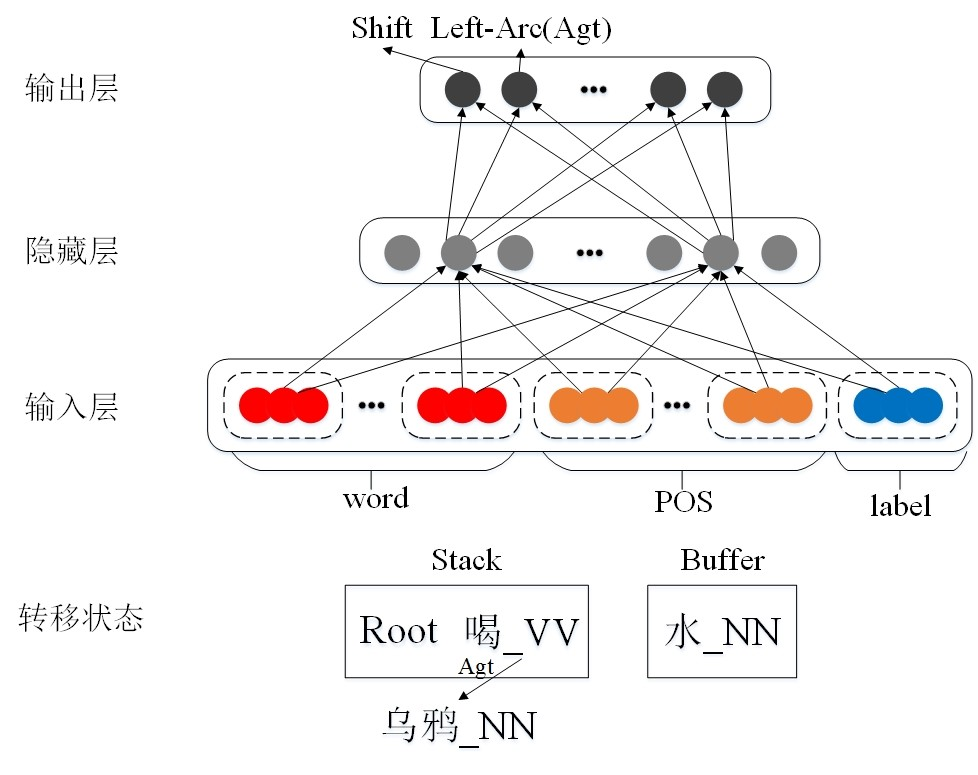
\includegraphics[width=80mm]{picture/chen2014mlp.jpg}
	\caption{作为基于转移的依存分析分类器的MLP}
	\label{fig:chen2014mlp}
\end{figure}

受到该工作的启发,我们在录用于CCL 2016的工作中也使用了MLP作为分类器,有效解决了上述几个问题。首先,由于对词向量的初始化使用了用大规模语料预先训练得到的词向量,其中包含的词比训练语料中出现的词要多很多,一定程度上缓解了数据稀疏问题。其次,神经网络中采用三次方函数作为激活函数,避免了人工特征组合,而且对所有隐层节点特征进行三三组合,对特征组合的覆盖更全面。最后,神经网络中使用低维稠密的向量形式表示词、词性和依存弧特征,避免了特征字符串组合的过程,大大缩短了分析所需时间。然而在该方法中仍然只选择了转移系统中有限的一些位置的特征向量作为预测的依据,还有大量位置未被考虑,而这些位置却可能包含了长距离依赖等对于依存分析十分重要的信息。

\citeayu{dyer-EtAl:2015:ACL-IJCNLP}提出了Stack LSTM结构,用几个单向LSTM分别计算转移系统中每部分所有信息的表示向量,然后将这些向量组合起来作为当前转移状态的表示$e_t$:

\vspace{-0.6em}
\begin{equation}
e_t=\max(0,W[s_t\oplus b_t \oplus p_t \oplus a_t ]+d)
\end{equation}

其中$W$是参数矩阵,$s_t$是Stack LSTM对$\sigma$的编码,$b_t$是Stack LSTM对$\beta$的编码, $p_t$是Stack LSTM对$\delta$的编码,$a_t$是Stack LSTM对$A$的编码,$d$是偏置项。
之后转移状态$e_t$用于计算该状态下转移动作的概率分布:

\vspace{-0.6em}
\begin{equation}
p(z_t|e_t)=\frac{\exp(g^T_{z_t}e_t + q_{z_t})}{\sum_{z'\in A(\sigma, \beta)}\exp (g^T_{z'}e_t+q_{z'})}
\end{equation}

其中$g_z$是用于表示转移动作$z$的列向量,而$q_z$是其偏置项,集合$A(\sigma,\beta)$是在当前状态下可以执行的转移动作。

为了获取对转移状态更全面的表示,我们在该结构的基础上提出了2个有效的神经网络模块,即Bi-LSTM Subtraction和Incremental Tree-LSTM,分别对转移过程中的缓存和子图进行建模,因此我们最终的依存图分析系统简称为BS-IT系统。图~\ref{fig:bsit}给出了我们提出的模型的整体结构图。接下来分别对两个模块进行具体介绍。

\begin{figure}[hbtp]
	\centering
	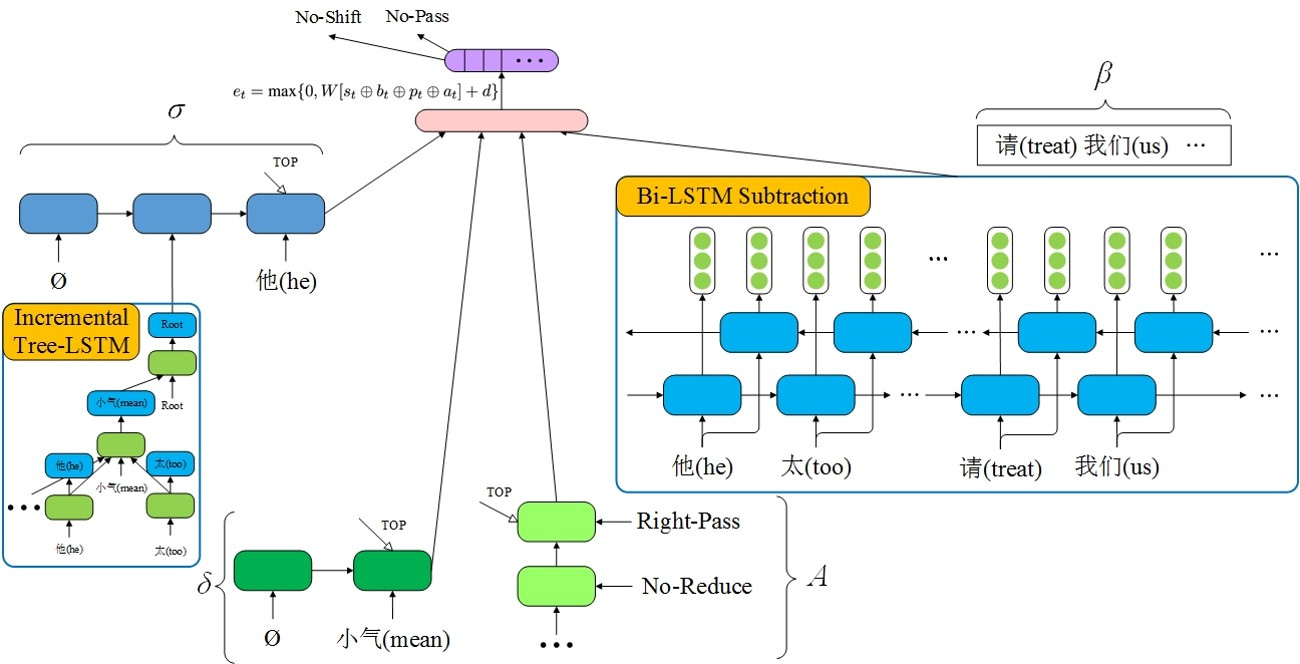
\includegraphics[width=130mm]{picture/bsit.jpg}
	\caption{BS-IT系统模型整体结构图}
	\label{fig:bsit}
\end{figure}

\citeayu{dyer-EtAl:2015:ACL-IJCNLP}的模型中简单地使用从右向左的单向LSTM的最后一个隐层状态向量表示缓存中的所有信息。这种方法不但无法获取缓存之外的词(已被移入栈中或规约)的信息,也损失了从左向右的上下文信息。而且,我们认为只用一个隐层状态向量是无法很好地表示整个缓存中的信息的。

\begin{figure}[hbtp]
	\centering
	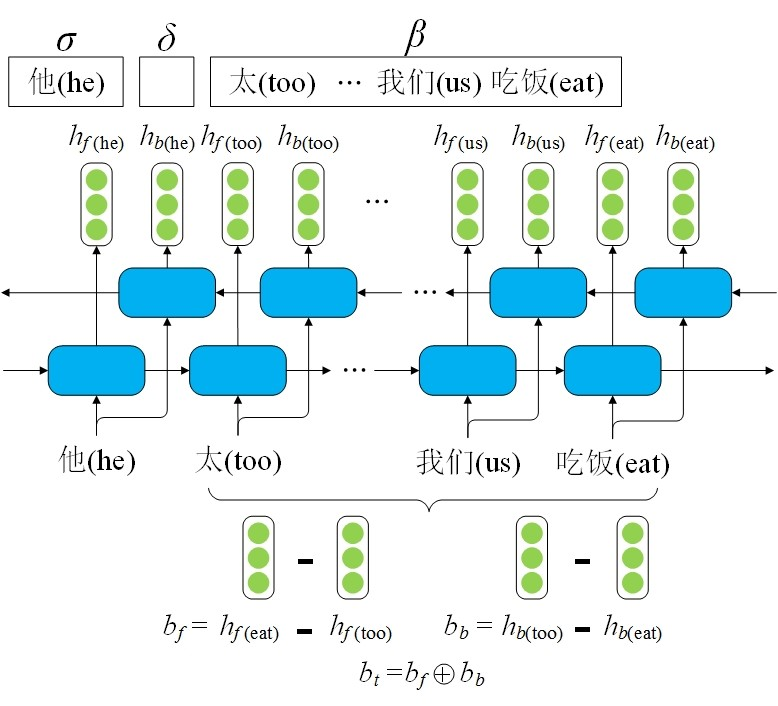
\includegraphics[width=80mm]{picture/bs.jpg}
	\caption{Bi-LSTM Subtraction模块结构图}
	\label{fig:bs}
\end{figure}

\citeayu{wang-chang:2016:P16-1,cross-huang:2016:EMNLP2016}探索了使用LSTM两个时间节点的隐层输出之差表示这两个节点中间的一段信息的方式,证明了该方法的有效性。
类似的,我们将缓存看作一个段,并用段头和段尾的表示的差来表示整个段。
在句法依存分析领域,许多近期工作\citeyqy{wang-EtAl:2016:N16-12,kiperwasser2016simple,cross-huang:2016:P16-2}都将词、词性的向量输入双向LSTM中,然后用其隐层输出代替原来的词、词性向量表示句中的词,从而在词的表示中包含上下文信息。
因此,为了获得缓存之外词的信息,我们首先将整个句子输入双向LSTM中,用每个词对应的隐层状态向量作为其表示。我们将该模块命名为Bi-LSTM Subtraction。

我们用以下公式计算整个缓存在$t$时刻的表示$b_t$:

\begin{equation}
b_f=h_f(l)-h_f(f)
\end{equation}
\begin{equation}
b_b=h_b(f)-h_b(l)
\end{equation}
\begin{equation}
b_t=b_f \oplus b_b
\end{equation}

其中,$l$和$f$分别表示在$t$时刻缓存$\beta$中最左边的词和最右边的词,$h_f(a)$和$h_b(a)$分别表示词$a$在从左向右和从右向左的LSTM中的隐层输出。

例如图~\ref{fig:bs}中计算缓存的表示时,先用“吃饭”的正向LSTM表示$h_f(eat)$减去“太”的正向LSTM表示$h_f(too)$,获得该段正向的表示,再用“太”的反向LSTM表示$h_b(too)$减去“吃饭”的反向LSTM表示$h_b(eat)$,获得该段反向的表示。二者拼接起来作为此时缓存的表示。

\citeayu{dyer-EtAl:2015:ACL-IJCNLP}的模型中使用基于依存的递归神经网络(RecNN)\citeyqy{socher2011parsing}来计算转移过程中的子结构,在处理较深的子结构时,这种方法可能会遇到梯度消失问题。为了解决该问题,我们利用Tree-LSTM\citeyqy{tai-socher-manning:2015:ACL-IJCNLP}对这些子结构进行建模。图~\ref{fig:it}显示了我们提出的Incremental Tree-LSTM与基于依存的RecNN的区别。RecNN通过递归地组合一个个父节点-子节点对来构建子图,而Tree-LSTM则能同时合并一个节点及其所有子节点。我们将该模块命名为Incremental Tree-LSTM。

\begin{figure}[hbtp]
	\centering
	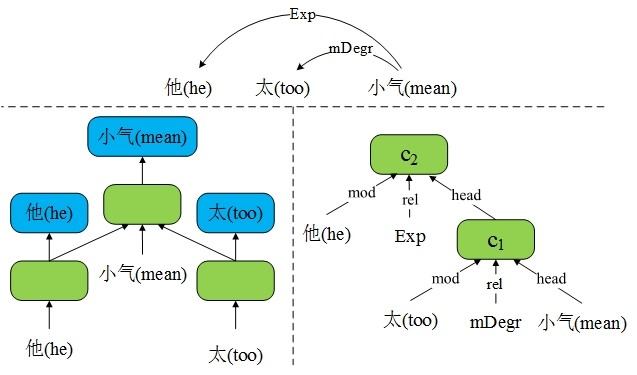
\includegraphics[width=80mm]{picture/it.jpg}
	\caption{Incremental Tree-LSTM模块结构图}
	\label{fig:it}
\end{figure}

由于基于转移的依存图分析的特点,我们使用的Tree-LSTM与一般的Tree-LSTM有两点不同。首先,显然该任务中需要建模的子结构不一定是树。但好在我们处理的依存图不包括环,因此仍然能够使用LSTM。更重要的是,与一般的Tree-LSTM能够同时获得一个节点的所有子节点不同,在基于转移的依存分析中,一个节点的子节点是逐个被找到的,因此我们需要不断利用Tree-LSTM更新父节点信息。具体来说,对于一个词,每当找到它的一个新子节点,就要将其所有已经找到的子节点和其本身的表示输入Tree-LSTM中计算它的新表示。例如,在图~\ref{fig:it}中,我们会首先找到“太”与“小气”之间的依存弧,这时需要用Tree-LSTM合并二者的表示向量并将其作为“小气”的新表示。然后我们会发现“小气”的另一个子节点“他”,这时需要用Tree-LSTM合并“他”和“小气”的表示,以及之前已经找到的“小气”的子节点“太”的表示,将这三者表示合并之后作为父节点“小气”的新表示。

通过增加上述两个神经网络模块,我们获得了转移系统中重要的缓存和子图的更有效的表示,从而提高了基于转移的依存图分析器的精度。这部分工作已被AAAI 2018录用。

\subsubsection{实验结果}

\begin{table}[htpb]
	\centering
	\begin{tabular}{l||cc|cc||cc|cc}
		\hline
		\multirow{2}{*}{\bf 系统}&\multicolumn{4}{c}{\bf NEWS}&\multicolumn{4}{c}{\bf TEXTBOOKS}\\
		\cline{2-9}
		&\bf LF&\bf UF&\bf NLF&\bf NUF&\bf LF&\bf UF&\bf NLF&\bf NUF\\
		\hline
		IHS-RD-Belarus&59.06&77.64&40.84&60.20&68.59&82.41&50.57&64.58\\
		OCLSP (lbpg)&57.22&74.93&45.57&58.03&65.54&79.39&51.75&63.21\\
		OCLSP (lbpgs)&57.81&75.54&41.56&54.34&66.21&79.85&47.79&55.51\\
		OCLSP (lbpg75)&57.78&75.40&48.89&58.28&66.38&79.91&57.51&63.87\\
		OSU\_CHGCG&55.69&73.72&49.23&60.71&65.17&78.83&54.70&65.71\\
		\hline
		MLP & 60.71&77.86&47.01&61.90&70.04&82.01&55.59&65.55 \\ 
		\hline
		2-stage & 62.29&80.56&39.93&64.29&71.94&85.24&50.67&69.97 \\ 
		\hline
		Basic&62.23&80.42&49.18&63.90&71.51&84.95&59.70&71.63\\
		BS-IT&\bf63.30&\bf81.14&\bf51.16&\bf66.92&\bf72.92&\bf85.71&\bf61.91&\bf72.74\\
		\hline
	\end{tabular}
	\caption{SemEval-2016 Task 9中文数据集上的实验结果}
	\label{tbl:result-semeval16}
	\vspace{-0.3em}
\end{table}

我们的系统在中英文数据集上都获得了很好的实验结果,表~\ref{tbl:result-semeval16}是SemEval-2016 Task 9中文数据集上的实验结果。该数据集分为两部分,分别是新闻集(NEWS)和小学课本集(TEXTBOOKS),前者句子较长、较复杂,后者句子较短、较简单。该评测的评价指标中最重要的两个分别是弧标签的F值(LF)和有多父节点的词的弧标签的F值(NLF)。

表中前5行是参加该评测的其它系统的结果,第6行是我们录用于CCL 2016的论文中使用MLP作为分类器的系统的结果,第7行是我们录用于AAAI 2018的论文中实现的一个两步的基准系统,该系统参考了\citeayu{ding2014chinese}的方法,首先用传统依存树分析器预测出依存树结构,然后用一个支持向量机(Support Vector Machine,SVM)作为分类器从一个由规则产生的候选弧集合中选出一些弧加入其中组合成语义依存图。为了方便比较,在第一步预测时使用了我们提出的BS-IT系统作为分类器。最后两行是我们录用于AAAI 2018的论文中提出了模型,其中Basic表示不使用Bi-LSTM Subtraction和Incremental Tree-LSTM两个模块时的结果,BS-IT表示同时使用这两个模块时的结果。实验结果显示我们提出的模型获得了该数据集上最好结果,尤其在对图结构评价至关重要的NLF值上相比原有方法有巨大提升。

\begin{table}
	\centering
	\begin{tabular}{l||ccc|c}
		\hline
		\bf 系统&\bf DM&\bf PAS&\bf PSD &\bf 宏平均\\
		\hline
		\multicolumn{5}{c}{\bf IN-DOMAIN}\\
		\hline
		\citeayu{du-EtAl:2015:SemEval} (ensemble) &89.1&91.3&75.7&85.4\\
		\citeayu{almeida-martins:2015:SemEval} (single) &88.2&90.9&76.4&85.2\\
		\citeayu{peng-thomson-smith:2017:Long} (single) &89.4&\bf 92.2&77.6&86.4\\
		\hline
		BS-IT (single) &89.3&91.4&76.1&85.6\\
		BS-IT (ensemble) &\bf 90.3& 91.7&\bf 78.6&\bf 86.9\\
		\hline
		\multicolumn{5}{c}{\bf OUT-OF-DOMAIN}\\
		\hline
		\citeayu{du-EtAl:2015:SemEval} (ensemble) &81.8&87.2&73.3&80.8\\
		\citeayu{almeida-martins:2015:SemEval} (single) &81.8&86.9&74.8&81.2\\
		\citeayu{peng-thomson-smith:2017:Long} (single) &84.5&\bf 88.3&75.3&82.7\\
		\hline
		BS-IT  (single) &83.2&87.2&73.2&81.2\\
		BS-IT (ensemble) &\bf 84.9&87.6&\bf 75.9&\bf 82.8\\
		\hline
	\end{tabular}
	\caption{SemEval-2015 Task 18英文数据集上的实验结果,single表示单模型,ensemble表示模型融合方法。}
	\label{tbl:result-semeval15}
\end{table}

此外,我们还在SemEval-2015 Task 18英文广义语义依存图数据集上测试了我们的模型,该数据集一共有三种标注规范(DM、PAS和PSD),每种规范都有两部分测试数据集,即同领域(IN-DOMAIN)与不同领域(OUT-OF-DOMAIN)测试数据。表~\ref{tbl:result-semeval15}中\citeayu{du-EtAl:2015:SemEval}和\citeayu{almeida-martins:2015:SemEval}是参加该评测的系统,前者是利用了多个不同的基于转移和基于图的模型同时预测并对最终结果进行投票,后者是一个基于图的方法,利用了$AD^3$算法进行解码。\citeayu{peng-thomson-smith:2017:Long}也是一个基于图的方法,他们同时利用三种标注体系进行多任务学习,取得了该数据集上最好结果,这里列出的是他们没有使用多任务学习的基础模型结果。BS-IT是我们的系统结果。受到\citeayu{du-EtAl:2015:SemEval}的启发,我们也使用了一个简单的模型融合方法,在训练时使用不同随机初始化种子训练多个模型。在预测时,用这些模型算出的分数之和来选择接下来的转移动作。实验证明该方法有效提高了系统性能,从而达到与该数据集上最好结果相近的结果。
